\documentclass[11pt]{cernrep}
\usepackage{graphicx,epsfig}
\usepackage{amsmath}
\bibliographystyle{lesHouches}

% definitions here, only use \newcommand, no \def
\newcommand{\order}{\ensuremath{\mathcal{O}}}
\newcommand{\alphas}{\ensuremath{\alpha_\mathrm{s}}}
\newcommand{\rd}{\ensuremath{\mathrm{d}}} % differential
\newcommand{\ri}{\ensuremath{\mathrm{i}}} % imaginary i
\newcommand{\re}{\ensuremath{\mathrm{e}}} % exp != elem. charge
\newcommand{\rT}{\ensuremath{\mathrm{T}}} % transverse

% labels in math formulae
\newcommand{\rLO}{\ensuremath{\mathrm{LO}}}
\newcommand{\rNLO}{\ensuremath{\mathrm{NLO}}}
\newcommand{\rNNLO}{\ensuremath{\mathrm{NNLO}}}
\newcommand{\rQCD}{\ensuremath{\mathrm{QCD}}}
\newcommand{\rEW}{\ensuremath{\mathrm{EW}}}
\newcommand{\rYFS}{\ensuremath{\mathrm{YFS}}}
\newcommand{\rSherpa}{\ensuremath{\mathrm{Sherpa}}}
\newcommand{\rPA}{\ensuremath{\mathrm{PA}}}

% heppennames-like particle macros
%% bosons
\DeclareRobustCommand{\PZ}{{\ensuremath{\mathrm{Z}}}}
\DeclareRobustCommand{\PWpm}{{\ensuremath{\mathrm{W}^{\pm}}}}
%% leptons
\DeclareRobustCommand{\Pl}{{\ensuremath{\ell}}}
\DeclareRobustCommand{\Pal}{{\ensuremath{\bar{\ell}}}}
\DeclareRobustCommand{\Plp}{{\ensuremath{\ell^+}}}
\DeclareRobustCommand{\Plm}{{\ensuremath{\ell^-}}}
%% nucleons
\DeclareRobustCommand{\Pp}{{\ensuremath{\mathrm{p}}}}


\begin{document}

% find a catchy title, this is just a filler
\title{Electroweak corrections in Drell--Yan production}

\author{
  A.\ Huss$^{1,2}$,
  M.\ Sch\"onherr$^2$
}
\institute{
  $^1$ Institute for Theoretical Physics, ETH, CH-8093 Z\"urich, Switzerland \\
  $^2$ Department of Physics, University of Z\"urich, CH-8057
  Z\"urich, Switzerland
}

\maketitle

\begin{abstract}
  We compare the description of higher-order electroweak corrections at 
  $\order(\alpha)$ and $\order(\alphas\alpha)$ for the neutral-current 
  Drell--Yan process.
\end{abstract}


\section{Introduction}
\label{sec:dyew:intro}

%%%%% Motivation -> neutral-current DY
The Drell--Yan-like production of electroweak gauge bosons represents one of the key Standard Model processes at hadron colliders whose detailed understanding is crucial in order to exploit the full potential of the measurements performed at the LHC.
The neutral-current process $\Pp\Pp\to\PZ/\gamma\to\Plp\Plm$, in particular, has a very clean experimental signature owing to the two charged leptons in the final state which further allows for the full reconstruction of the kinematics of the intermediate gauge boson.
Not only does this process constitute a powerful tool for detector calibration, but it also delivers important constraints in the fit of PDFs and allows for precision measurements such as the extraction of the weak mixing angle $\sin^2(\theta^{\Pl}_\mathrm{eff})$.

%%%%% Theory status: fixed order
On the theory side, Drell--Yan production belongs to one of the most precisely predicted processes:
QCD corrections are known up to NNLO~~\cite{Hamberg:1990np,Harlander:2002wh,Anastasiou:2003ds,Melnikov:2006di,Melnikov:2006kv,Catani:2009sm,Gavin:2010az,Gavin:2012sy}, the electroweak~(EW) corrections up to NLO~\cite{Baur:1997wa,Zykunov:2001mn,Baur:2001ze,Dittmaier:2001ay,Baur:2004ig,Arbuzov:2005dd,CarloniCalame:2006zq,Zykunov:2005tc,CarloniCalame:2007cd,Arbuzov:2007db,Brensing:2007qm,Dittmaier:2009cr}, and many further improvements beyond fixed-order predictions (see, e.g., references in Ref.~\cite{Dittmaier:2015rxo}).
Until recently, the largest missing piece in terms of fixed-order predictions were given by the NNLO mixed QCD--EW corrections.
Different approaches of combining QCD and EW corrections revealed that the missing $\order(\alphas\alpha)$ corrections could have an impact of a few per cent in the resonance region, i.e.\ at the level that is relevant for precision phenomenology.
In a series of papers~\cite{Dittmaier:2014qza,Dittmaier:2015rxo}, the calculation of these corrections have been tackled using the so-called pole approximation~(PA).
This approach is suitable to describe observables that are dominated by resonances with sufficient accuracy.

%%%%% Some context
In this work, we investigate how the $\order(\alphas\alpha)$ corrections 
generated through a universal process-independent resummation approach 
compares to the results of Ref.~\cite{Dittmaier:2015rxo}.
Section~\ref{sec:dyew:comp} gives a brief overview of the computation 
employing the PA and the implementation of the QED shower in the 
\textsc{Sherpa} Monte Carlo program~\cite{Gleisberg:2008ta}.
In Sect.~\ref{sec:dyew:results} we present our numerical results of the 
comparison before we conclude in Sect.~\ref{sec:dyew:conclusions}.


\section{Computational setup}
\label{sec:dyew:comp}

%%%%% The pole approximation
\paragraph{The Pole approximation:}
The calculation of the $\order(\alphas\alpha)$ corrections presented in Refs.~\cite{Dittmaier:2014qza,Dittmaier:2015rxo} was performed in the framework of a pole expansion, which is based on a systematic expansion of the cross section around the gauge-boson resonance $p_V^2\sim\mu_V^2$, with $\mu_V^2=M_V^2-\ri M_V\Gamma_V$ denoting the gauge-invariant location of the propagator pole in the complex plane. 
Only retaining the leading contributions that are enhanced by a resonant propagator, we obtain the so-called pole approximation~(PA).
As a result of applying the PA, the calculation is split into separate well-defined parts that can be classified into the non-factorizable and factorizable corrections: 
The non-factorizable corrections involve soft-photon exchange between the production and decay stages of the process and constitute the conceptually most difficult part of the calculation.
They have been computed in Ref.~\cite{Dittmaier:2014qza} and were found to be negligible for all phenomenological purposes.
The factorizable contributions, on the other hand, involve corrections where the production of the intermediate gauge boson and its decay proceed independently. 
Here, the factorizable corrections of ``initial--final'' type were identified as the numerically dominant contribution---combining the sizeable QCD corrections to the production sub-process with the large EW corrections of the gauge boson decay---and were computed in Ref.~\cite{Dittmaier:2015rxo}.
The remaining factorizable corrections are given by the ``initial--initial'' and ``finial--final'' types.
The latter were found to be numerically negligible~\cite{Dittmaier:2015rxo}, while the former are not expected to deliver a sizeable correction, in particular for observables that are less sensitive to initial-state radiation effects.
In the remainder of this work, we will thus focus our attention to the initial--final factorizable corrections which we will often simply refer to as the $\order(\alphas\alpha)$ corrections in the PA.
More details on this calculation can be found in Refs.~\cite{Dittmaier:2014qza,Dittmaier:2015rxo}.

%%%%% Sherpa's YFS shower
\paragraph{The QED resummation in Sherpa:}
Another approach to higher order QED or electroweak corrections is 
presented in the soft-photon resummation of Yennie, Frautschi and 
Suura (YFS)~\cite{Yennie:1961ad}. Therein the universal structure 
of real and virtual soft photon emissions is exploited to construct 
an all-order approximation to the process at hand which can be 
systematically supplemented with process-dependent finite hard 
real and virtual emission corrections. The implementation presented 
in Ref.~\cite{Schonherr:2008av} focusses on higher-order QED corrections 
to particle decays and is used since as the default mechanism for such 
corrections in \textsc{Sherpa}~\cite{Gleisberg:2008ta}, both for 
elementary particle (e.g.\ $\PWpm$, $\PZ$, $\tau^\pm$) as well as 
hadron decays. 

In the present context of lepton pair production the higher-order 
QED corrections are effected in a factorised approach. The complete 
process $\Pp\Pp\to\Plp\Plm$ is calculated at LO or NLO in the strong 
coupling constant keeping all off-shell effects. Then, an intermediate 
resonance $X$ is reconstructed from the lepton pair and assigned its 
invariant mass. Its decay width is then corrected for higher order 
QED corrections, including YFS resummation, to 
\begin{equation}
  \begin{split}\label{eq:dyew:comp:yfs}
    \Gamma
    \,=\;&
      \frac{1}{2m_X}\sum\limits_{n_\gamma=0}^\infty\frac{1}{n_\gamma !}
      \int\rd\Phi\;\re^{Y(\Omega)}
      \prod\limits_{i=1}^{n_\gamma}\rd\Phi_i\,\tilde{S}(k_i)\,\Theta(k_i,\Omega)
      \left[
        \tilde\beta_0^0
        +\tilde\beta_0^1
        +\sum\limits_{i=1}^{n_\gamma}\frac{\tilde\beta_1^1(k_i)}{\tilde{S}(k_i)}
        +\order(\alpha^2)
      \right]\;.
  \end{split}
\end{equation}
Therein, $m_X$ is the mass of the decaying resonance and $\rd\Phi$ 
is the phase element of the leading order decay, and $\tilde\beta_0^0$ is 
the leading order decay squared matrix element. The $Y(\Omega)$ then 
is the sum of the eikonal approximations to virtual photon exchange and 
unresolved soft real photon emission, $\Omega$ denoting the region in which 
soft photons are not resolvable. The YFS form factor, $\re^{Y(\Omega)}$, then 
resums these leading logarithmic universal corrections to all orders. 
Resolved photons are then described explicitly, emission by emission, 
by the eikonal $\tilde{S}$ depending on the individual photon momentum 
$k_i$. $\rd\Phi_i$ is the corresponding phase space element. The 
eikonal approximations used in both the YFS form factor and for 
resolved real emissions can then, order-by-order, be corrected by 
supplementing the corresponding infrared-subtracted squared matrix 
elements $\tilde\beta_i^{i+j}$ of $\order(\alpha^{i+j})$ relative to 
the Born decay and containing $i$ resolved photons. Since all charged 
particles are considered massive in the context of YFS resummation, 
all $\tilde\beta_i$ are free of any infrared singularity. Finally, it is 
interesting to note that in the case of multi-photon emission 
each emitted photon receives the hard emission correction $\tilde\beta_1^1$ 
in the respective one-photon emission projected phase space.

The implementation used here, as we restrict the $\gamma^*/Z$ propagator 
virtuality to be near the $Z$ mass, always identifies the resonance $X$ with 
the $Z$ boson. The calculation thus contains the $\order(\alpha)$ virtual 
corrections $\tilde\beta_0^1$ and real emission corrections $\tilde\beta_1^1$ 
resulting in an NLO QED accurate description. As NLO weak corrections 
are finite they can in principle be incorporated in the $\tilde\beta_0^1$. 
This is left to a future work.


\section{Results}
\label{sec:dyew:results}

%%%%% numerical setup
The numerical results presented in this section are obtained using 
the same input parameters and event selection cuts as in 
Ref.~\cite{Dittmaier:2015rxo}. The electroweak coupling constant 
$\alpha$ is defined in the $G_\mu$-scheme, with the exception of 
the photonic corrections which use $\alpha(0)$ as their coupling. 
For the parton distribution functions we use the NNPDF2.3QED NLO PDF 
set~\cite{Ball:2012cx}, in particular also the LO predictions shown in 
the following were evaluated using this choice. For the charged 
leptons in the final state we consider two different reconstruction 
strategies: In the case of ``dressed'' electrons, we apply a photon 
recombination procedure in order to treat all collinear 
lepton--photon configurations inclusively, whereas in the ``bare'' 
muon setup no such recombination is performed. Further details on 
the calculational setup and the event reconstruction are given in 
Ref.~\cite{Dittmaier:2015rxo}.

%%%%% define delta
In order to establish the setup of the two computations, we first 
consider the relative $\order(\alpha)$ corrections by applying 
the YFS resummation in \textsc{Sherpa} to the LO prediction, 
$\sigma^{\rLO\otimes\rYFS}$, and compare it to the full 
EW corrections denoted as $\sigma^{\rNLO[\rEW]}$%
\footnote{
  A comparison of the PA at $\order(\alpha)$ against the full 
  NLO EW corrections has been performed in Ref.~\cite{Dittmaier:2014qza}.
}.
The respective relative correction factors, normalised to the LO 
prediction, are then given by
\begin{align}
  \label{eq:dyew:delta:nlo}
  \delta_\alpha^\rYFS &= 
  \frac{\sigma^{\rLO\otimes\rYFS} - \sigma^\rLO}{\sigma^\rLO}
  , &
  \delta_\alpha &= 
  \frac{\sigma^{\rNLO[\rEW]} - \sigma^\rLO}{\sigma^\rLO}
  .
\end{align}
Please note, the thus defined $\delta_\alpha^\rYFS$ retains also 
higher orders of $\alpha$ contrary to $\delta_\alpha$. For the 
mixed QCD--EW corrections, we generate terms of $\order(\alphas\alpha)$ 
by applying the YFS resummation on top of the fixed-order NLO QCD 
prediction, which we denote by $\sigma^{\rNLO[\rQCD]\otimes\rYFS}$.
These results are compared to the best prediction of 
Ref.~\cite{Dittmaier:2015rxo}, $\sigma^{\rNNLO[\rQCD\times\rEW]}_{\rPA}$, 
which includes the full NLO QCD and EW corrections, supplemented by 
the dominant $\order(\alphas\alpha)$ corrections in the PA. In order 
to extract the genuine $\order(\alphas\alpha)$ contribution from the 
prediction based on the YFS resummation, we define the relative 
correction factor as follows,
\begin{align}
  \label{eq:dyew:delta:nnlo:yfs}
  \delta_{\alphas\alpha}^\rYFS &= 
  \frac{ (\sigma^{\rNLO[\rQCD]\otimes\rYFS} - \sigma^{\rNLO[\rQCD]}) 
        -(\sigma^{\rLO\otimes\rYFS} - \sigma^\rLO)}
       {\sigma^\rLO} .
\end{align}
For the fixed-order prediction in the PA, the corresponding correction 
factor is given by
\begin{align}
  \label{eq:dyew:delta:nnlo:pa}
  \delta_{\alphas\alpha}^\rPA &= 
    \frac{\sigma^{\rNNLO[\rQCD\times\rEW]}_{\rPA} - \sigma^{\rNLO[\rQCD+\rEW]}}
       {\sigma^\rLO} .
\end{align}
Again, as in Eq.~\ref{eq:dyew:delta:nlo}, $\delta_{\alphas\alpha}^\rYFS$ 
also contains higher orders in $\alpha$, contrary to 
$\delta_{\alphas\alpha}^\rPA$.

%%%%%%%%%%%%%%%%%%%%
\begin{figure}
  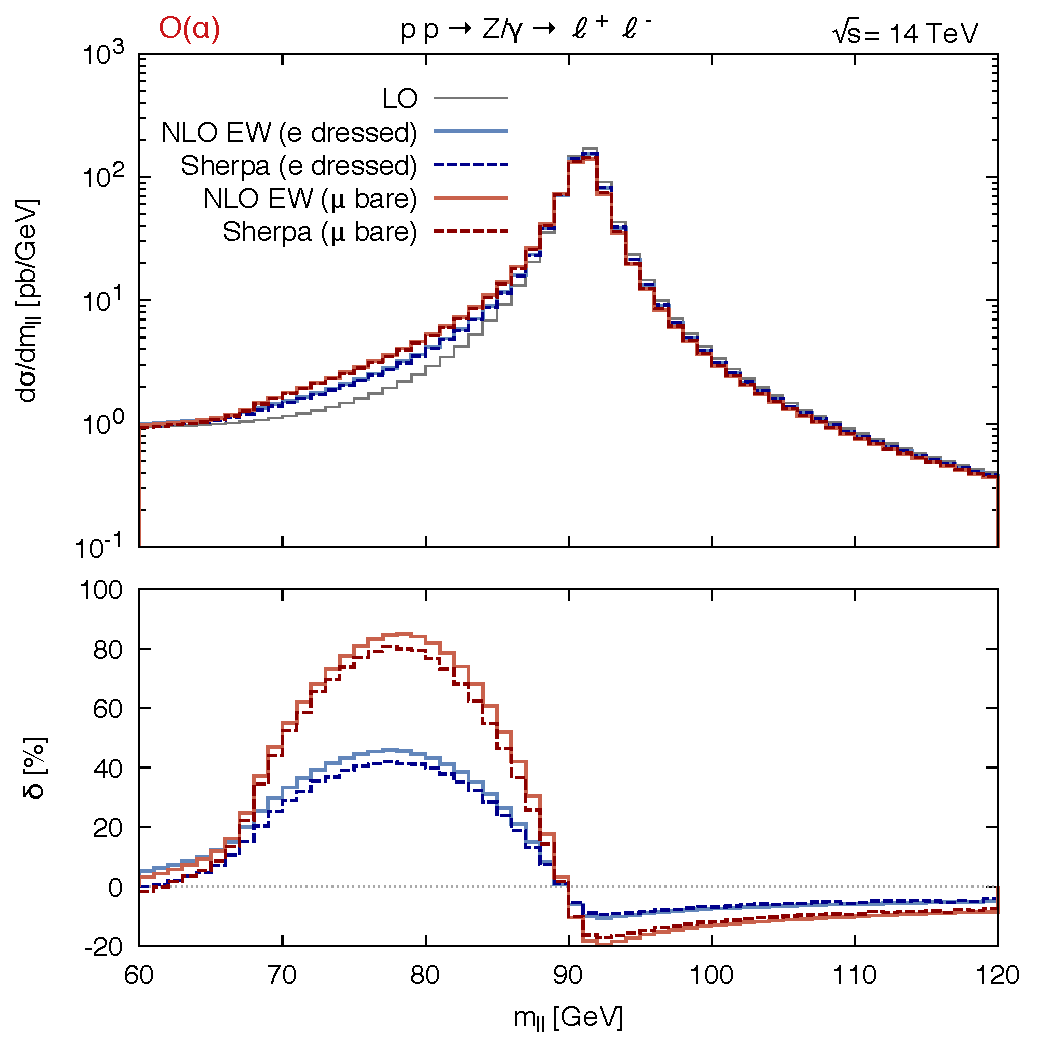
\includegraphics[width=.48\linewidth]{images/Z_mll2_LO.pdf} \hfill
  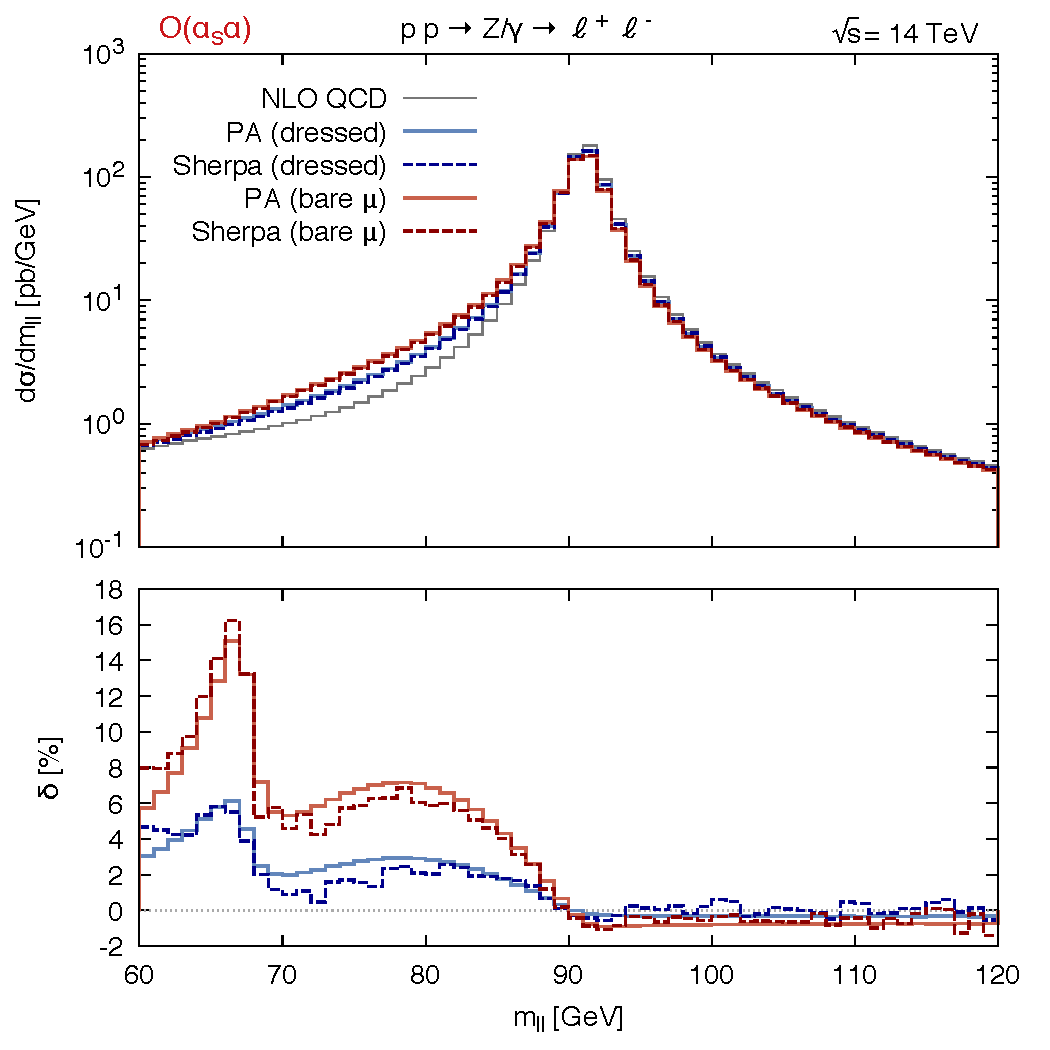
\includegraphics[width=.48\linewidth]{images/Z_mll2_NLO.pdf} 
  \caption{
    Comparison of the $\order(\alpha)$~(left) and $\order(\alphas\alpha)$ 
    (right) corrections to the invariant-mass distribution of the lepton 
    pair $m_{\Pl\Pl}$ between Ref.~\cite{Dittmaier:2015rxo} and Sherpa. 
    The absolute distributions and the relative corrections at the 
    respective order are shown in the top and bottom panels, respectively. 
    Collinear lepton--photon configurations are treated both inclusively 
    with a recombination procedure resulting in the ``e dressed'' setup 
    (blue) or exclusively in the case of muons labelled as ``$\mu$ bare'' 
    (red).
  }
  \label{fig:dyew:mll}
\end{figure}
%%%%%
\begin{figure}
  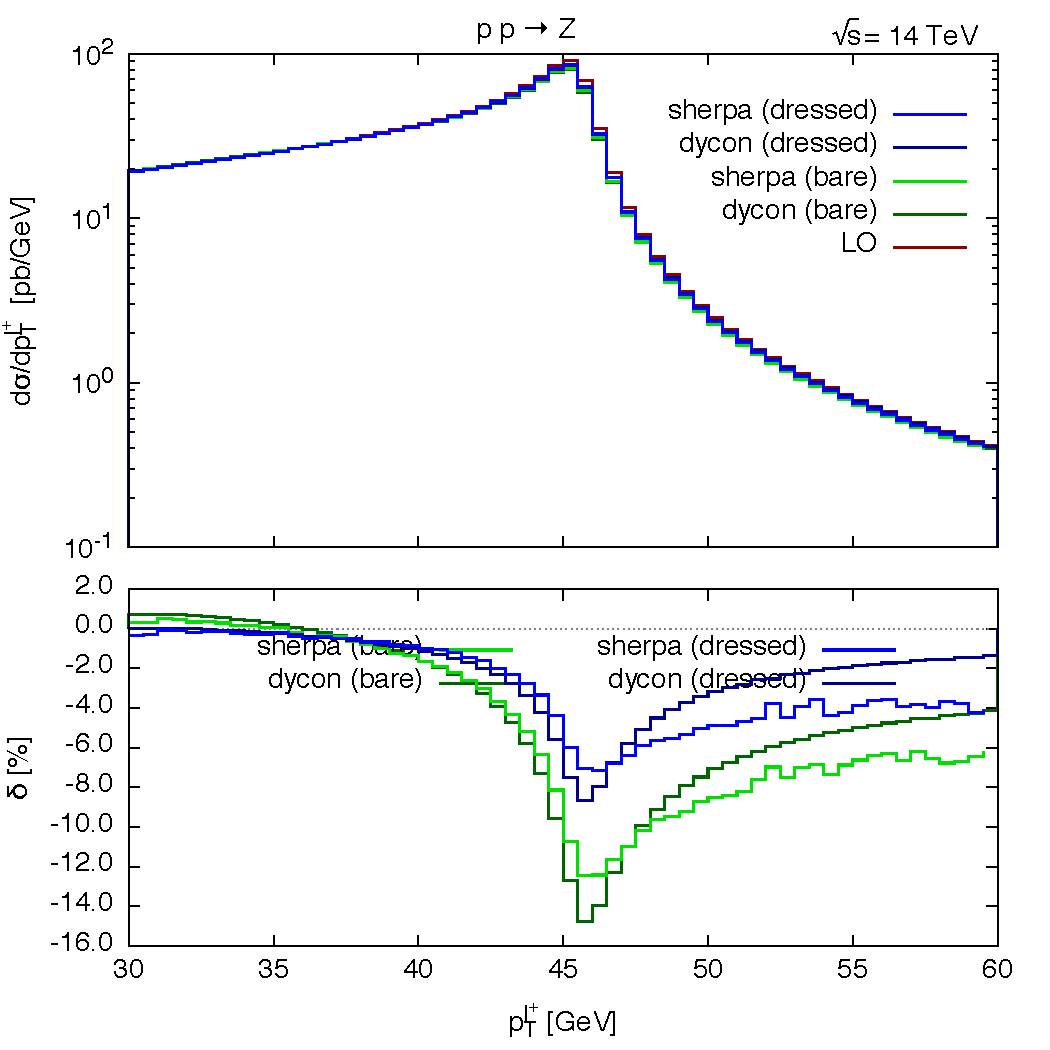
\includegraphics[width=.48\linewidth]{images/Z_ptl+2_LO.pdf} \hfill
  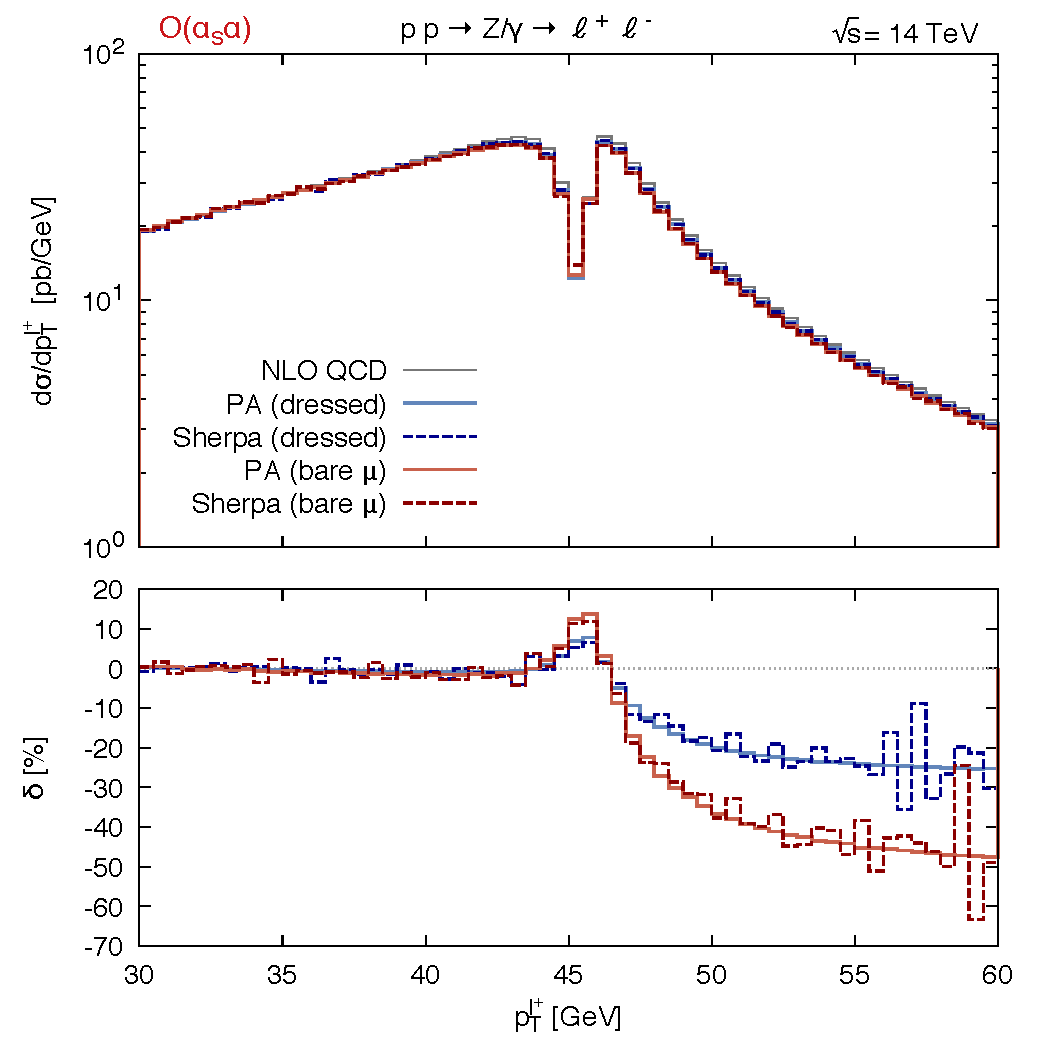
\includegraphics[width=.48\linewidth]{images/Z_ptl+2_NLO.pdf} 
  \caption{
    Comparison of the $\order(\alpha)$~(left) and $\order(\alphas\alpha)$ 
    (right) corrections to the transverse-momentum distribution of the 
    positively charged lepton $p_\rT^\Plp$ between 
    Ref.~\cite{Dittmaier:2015rxo} and Sherpa. The absolute distributions 
    and the relative corrections at the respective order are shown in the 
    top and bottom panels, respectively. Collinear lepton--photon 
    configurations are treated both inclusively with a recombination 
    procedure resulting in the ``e dressed'' setup~(blue) or exclusively in 
    the case of muons labelled as ``$\mu$ bare''~(red).
  }
  \label{fig:dyew:ptl}
\end{figure}
%%%%%
\begin{figure}
  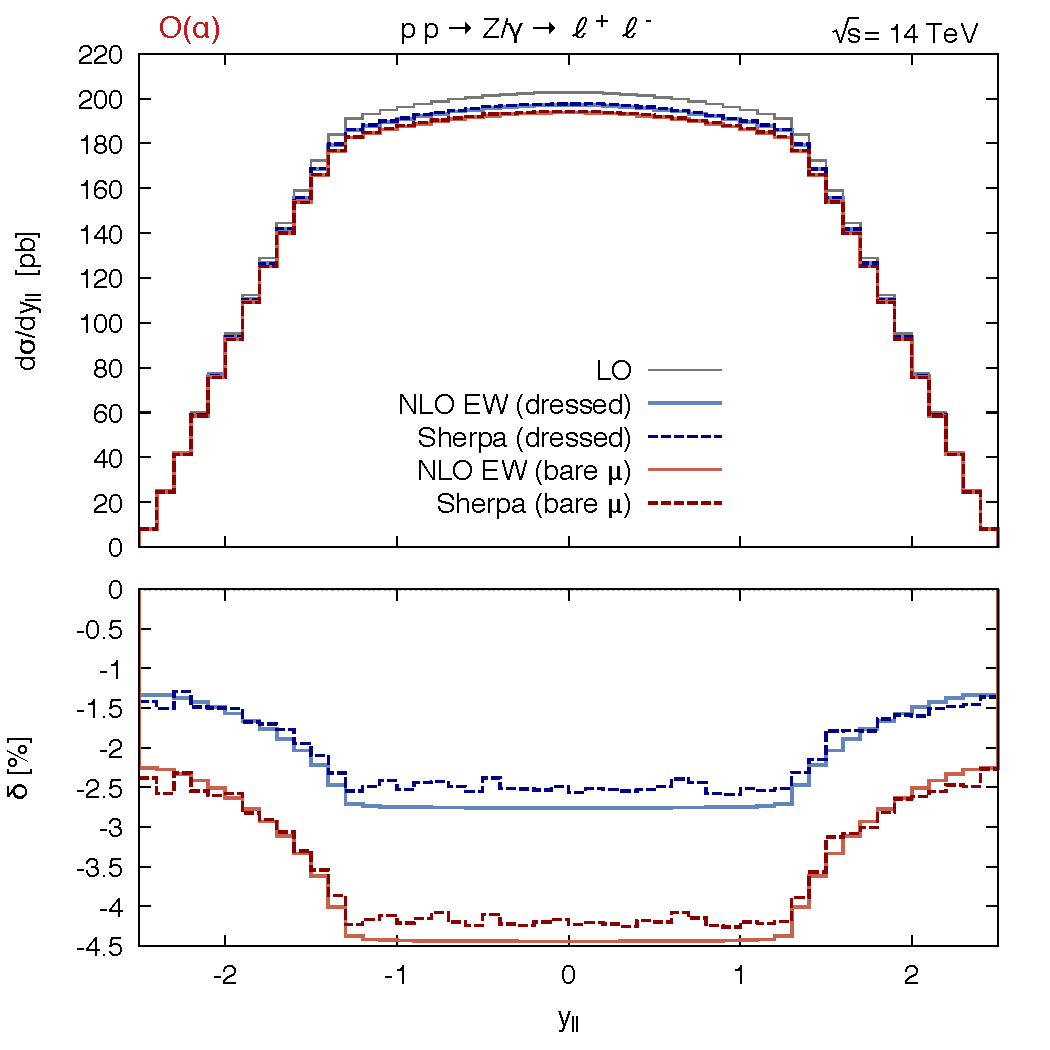
\includegraphics[width=.48\linewidth]{images/Z_yll_LO.pdf} \hfill
  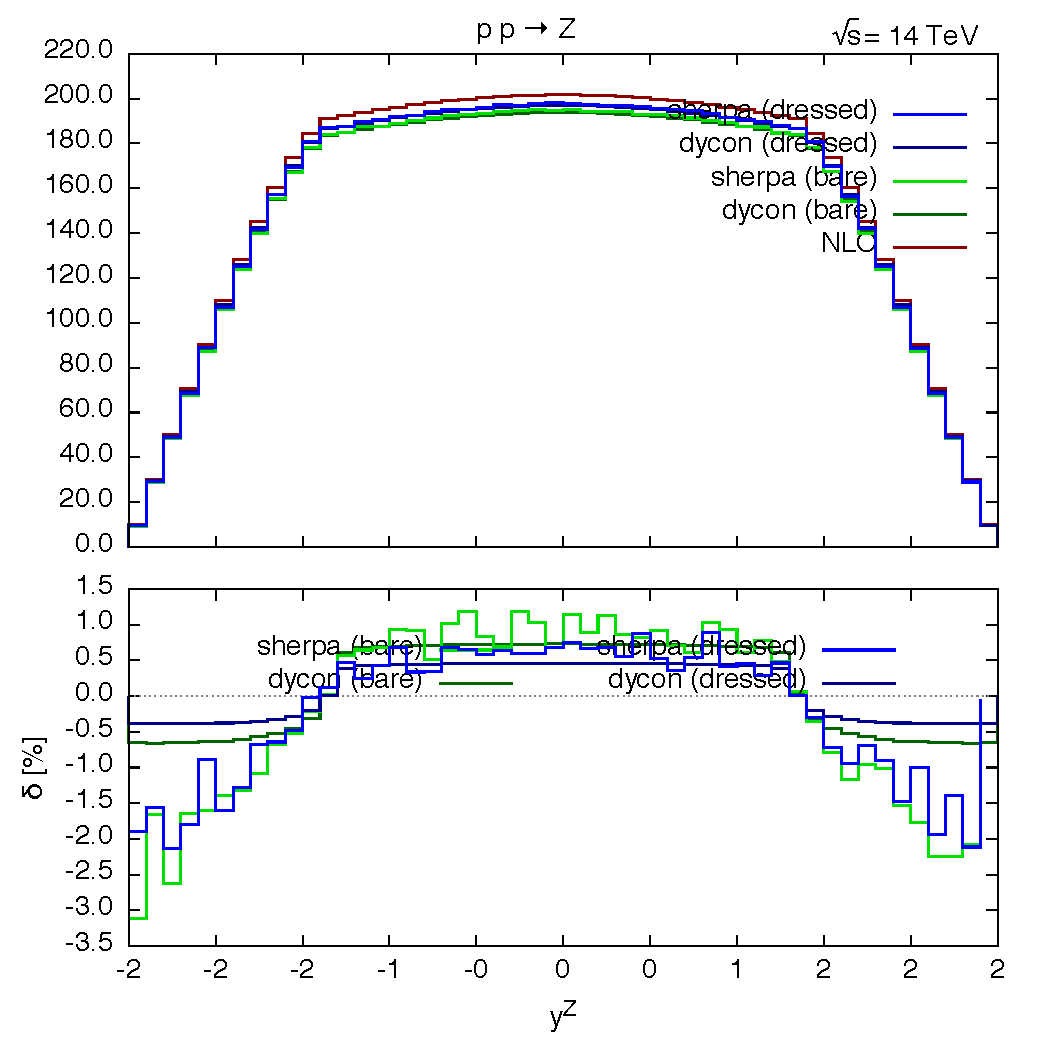
\includegraphics[width=.48\linewidth]{images/Z_yll_NLO.pdf}
  \caption{
    Comparison of the $\order(\alpha)$~(left) and $\order(\alphas\alpha)$ 
    (right) corrections to the rapidity distribution of the lepton pair 
    $y_{\Pl\Pl}$ between Ref.~\cite{Dittmaier:2015rxo} and Sherpa. The 
    absolute distributions and the relative corrections at the respective 
    order are shown in the top and bottom panels, respectively. Collinear 
    lepton--photon configurations are treated both inclusively with a 
    recombination procedure resulting in the ``e dressed'' setup~(blue) or 
    exclusively in the case of muons labelled as ``$\mu$ bare''~(red).
  }
  \label{fig:dyew:yll}
\end{figure}
%%%%%%%%%%%%%%%%%%%%


%%%%% discuss results
The numerical results comprise differential distributions in the 
lepton invariant mass $m_{\Pl\Pl}$, the transverse momentum of the 
positively charged lepton $p_\rT^\Plp$, and the rapidity of the 
lepton pair $y_{\Pl\Pl}$, which are shown in 
Figs.~\ref{fig:dyew:mll}--\ref{fig:dyew:yll}, respectively. The left plot 
in the figures shows a comparison of the $\order(\alpha)$ corrections, 
while the right-hand plot compares the corresponding $\order(\alphas\alpha)$ 
corrections. In each plot we show the absolute distributions in 
the top frame and the relative correction factors in the bottom 
panel as defined in Eq.~\eqref{eq:dyew:delta:nlo} for the $\order(\alpha)$ 
and Eqs.~\eqref{eq:dyew:delta:nnlo:yfs} and \eqref{eq:dyew:delta:nnlo:pa} 
for the mixed QCD--EW corrections.

%% mll
For the invariant mass distribution shown in Fig.~\ref{fig:dyew:mll} we 
observe an overall good agreement between the YFS resummation and 
the fixed-order result. This reflects the property of this observable 
whose corrections are known to be dominated by final-state photon 
emission. Both at $\order(\alpha)$ and $\order(\alphas\alpha)$ we 
observe a small offset between the two predictions where the resummed 
approach leads to slightly smaller corrections below the $\PZ$ 
resonance. This difference originates from multi-photon emissions, 
which is included in the YFS formalism, cf.\ Eq.~\eqref{eq:dyew:comp:yfs}, 
whereas the fixed-order prediction is restricted to at most one 
photon emission.
%% ptlp
Figure~\ref{fig:dyew:ptl} shows the corrections to the transverse momentum 
distribution of the positively charged lepton, $p_\rT^\Plp$. Although 
qualitatively displaying a similar shape in the $\order(\alpha)$ corrections, 
we observe larger differences between the two computations around the 
resonance and in the higher transverse momentum tails. This difference 
can be understood from the fact that this observable is sensitive to 
recoil effects from initial-state radiation which are not accounted for 
in the YFS approach as used here.  Indeed, comparing the final-state 
factorizable $\order(\alpha)$ corrections in PA to the full NLO EW 
corrections, as it is done in Fig.~9 in Ref.~\cite{Dittmaier:2014qza},
a very similar behaviour can be observed.
For the mixed QCD--EW corrections, on 
the other hand, the EW corrections contained in the 
$\order(\alphas\alpha)$ PA prediction are confined to the decay 
sub-process similarly to the case of the YFS resummation. As a result, 
we see a much better agreement between the two computations here.
%% yll
Lastly, the numerical results for the rapidity distribution of the 
lepton pair, $y_{\Pl\Pl}$, are shown in Fig.~\ref{fig:dyew:yll}. At 
$\order(\alpha)$, the resummed prediction is able to reproduce the 
exact fixed-order result to a large extent up to a small offset in 
the normalisation. This shift can be attributed to the finite weak 
corrections which are missing in the YFS resummed prediction here. 
The purely weak corrections amount to a flat correction of 
approximately $-0.5\%$ in this distribution as can be read off from
Fig.~14 in Ref.~\cite{Dittmaier:2009cr} and matches well with 
the observed offset. For the mixed QCD--EW corrections we obtain 
corrections from the YFS resummation that are similar in shape to 
those of the fixed-order prediction in the PA, however, with larger 
negative corrections in the forward regime which possibly stem from 
multi-photon effects on the event acceptance in this region.



\section{Conclusions and outlook}
\label{sec:dyew:conclusions}

%%%%% short summary
The Drell--Yan process is one of the most important ``standard candle'' 
processes at the LHC and, as such, has a wide range of applications.
In this work, we have explored the possibility of generating mixed 
QCD--EW corrections of $\order(\alphas\alpha)$ to this process using 
the YFS resummation available in the \textsc{Sherpa} Monte Carlo and 
performed a comparison to the fixed-order calculation of 
Ref.~\cite{Dittmaier:2015rxo}. To this end, we have considered both 
$\order(\alpha)$ and $\order(\alphas\alpha)$ corrections to various 
differential distributions given by the invariant mass of the leptons, 
the lepton transverse momentum, and the rapidity of the lepton pair.
We find that the QED resummation is able to capture the electroweak 
corrections to these observables remarkably well.
Furthermore, we were able to identify various sources for the differences 
that were observed between the two predictions.

%%%%% outlook
Building on the insights that were gained from this study, it will 
be interesting to investigate further observables and also repeating 
this comparison for the charged-current process. Potential 
improvements were identified in both computations which should be 
explored in order to gain further insights into the numerical impact of 
the various ingredients that enter the two predictions. Such 
improvements include the finite weak corrections that can be 
incorporated to the YFS approach through the $\tilde{\beta}^1$ 
coefficient in Eq.~\eqref{eq:dyew:comp:yfs} on the one side, and 
supplementing the fixed-order calculation with multi-photon emission 
effects. 


\section*{Acknowledgements}

We would like to thank the Les Houches workshop for hospitality offered 
during which some of the work contained herein was performed. 
A.H. acknowledges support from the ERC Advanced Grant MC@NNLO (340983). 
MS acknowledges support by the Swiss National Science Foundation (SNF) 
under contract PP00P2-128552.

%=================================
\bibliography{dyew_bib}
\end{document}
